\documentclass[main.tex]{subfiles}

\begin{document}

For a potential beta decay shape measurement, several criteria for a nucleus are needed.
The first is that the nucleus and the decay mode must be available in sufficient quantities that a proper decay spectrum shape can be measured.
This means that the nucleus needs to be relatively close to stability.
The decay mode needs to be clean.
If there are several competing decay modes of similar strength, the shape of the beta decay spectrum gets complicated.
The same thing happens if there are several gamma rays in the decay. 
Having one gamma ray is useful, as a coincidence measurement can be used to exclude much of any background spectra in the measurement.
In order to get a useful theoretical interpretation of the measurement of the Fierz term, a purely Fermi or Gamow-Teller transition is needed.
The superallowed decays are purely Fermi, so the limit on any potential scalar couplings is strong.
An allowed Gamow-Teller transition gives sensitivity to any potential couplings. 
A nucleus that fulfills these criteria is $^{20}$F. 
 
\section{$^{20}$F Decay Characteristics}
The decay scheme is given in figure \ref{fig:DecayScheme}.

\begin{figure}[!htb]
	\centerline{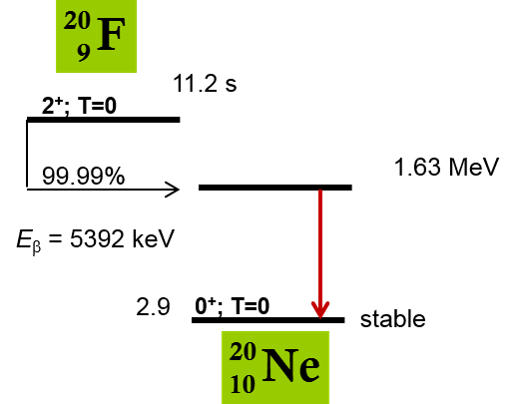
\includegraphics[width=0.78\textwidth]{20FDecayScheme.png}}
	\caption{The decay scheme of $^{20}$F.}
	\label{fig:DecayScheme}
\end{figure}

As seen in the figure, $^{20}$F decays 99.999\% of the time to the first excited state of $^{20}$Ne.
This decay is very clean, as there are very few contaminants from other decay branches. 
The $2^{+}$ state seen in the decay scheme is not the isobaric analogue state to the ground state of $^{20}$F.
That state is much higher in energy.
The beta decay therefor has a isospin change of 1.
This means that the allowed Fermi matrix element is zero, and the decay is an allowed Gamow-Teller transition. 
The forbidden transitions contribute <INSERT THEORY HERE> 
The half-life of $^{20}$F is about 11 seconds. 
This means waiting for the $^{20}$F to decay will take less than a minute to get good statistics.

The 1.6 MeV gamma ray in the transition allows for a coincidence measurement to take place.
One gamma ray does not distort the spectrum enough to cause any issues.
$^{20}$F is relatively close to stability. 
It can be made in sufficient qualities to get a good beta quality beta spectrum.
Because of these characteristics, this measurement was not the first to measure $^{20}$F.

\section{Previous Measurments of $^{20}$F}

Some of the earliest measurements of $^{20}$F where $ft$ value measurements \cite{Wil70} \cite{Alb75}.
The half-lives were measured with a plastic-scintillator in either case.  
These $ft$ values were compared to the mirror nucleus $^{20}$Na in order to search for second class currents in beta decay. 

Another, more recent measurement whose goal was putting limits on second class currents was done with with a polarized $^{20}F and $^{20}$Na beam \cite{Min11}.
The technique was an alignment measurement over different energies instead of an $ft$ value. 
The $^{20]$F was made with a polarized deuteron beam impinging on a $^{19}$F target. 
The direction of the outgoing electron was measured and recorded.
The angular distribution was measured using the beta-nuclear magnetic resonance (NMR) technique.
The correlations were corrected for and plotted vs energy.
The outcome of this graph was a measurement of the various form factors that correct the beta decay spectrum shape. 
The resulting $^{20}$F energy spectrum is shown in figure \ref{fig:keispec}

\begin{figure}[!htb]
	\centerline{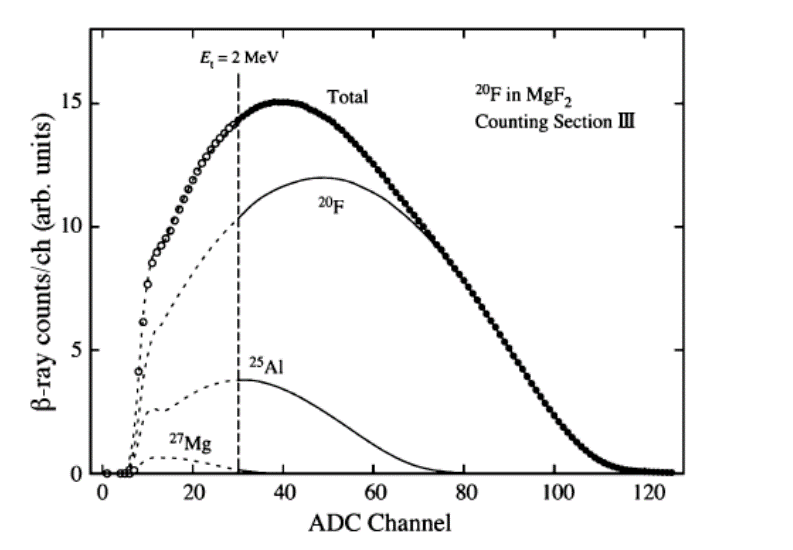
\includegraphics[width=0.78\textwidth]{Kei1120FSpectrum.png}}
	\caption{A sample beta energy spectrum using a beta-NMR technique \cite{Min11}}
	\label{fig:keispec}
\end{figure}

In the energy spectrum in figure \ref{fig:keispec}, there are several background spectra. 
Since this measurement  was an asymmetry measurement, the influence of the backgrounds are reduced. 

A shape measurement \cite{Het89} with a scintillator.

A shape measurement \cite{Elm87} with a spectrometer.
%Spectrum is on page 168 in thesis. Put it here

In order to get at the Fierz term, the beta decay spectrum shape must be described precisely.
The next chapter deals with the corrections to the beta decay spectrum.  

\end{document}
